
\section{Distribuciones continuas avanzadas}

En esta sección estudiaremos tres distribuciones continuas fundamentales y una herramienta
clave para analizarlas: la funci\'on generadora de momentos.

\subsection{Distribuci\'on uniforme continua}

La distribuci\'on uniforme continua modela el caso en el que una variable aleatoria toma
valores en un intervalo $[a,b]$ con la misma \emph{densidad} de probabilidad en todo punto.

\begin{definicion}[Distribuci\'on uniforme continua]
Una variable aleatoria continua $X$ tiene \emph{distribuci\'on uniforme continua} en el
intervalo $[a,b]$, con $a<b$, si su funci\'on de densidad est\'a dada por
\begin{align}
 \label{eq:2.8.1}
 f(x) =
 \begin{cases}
  \dfrac{1}{b-a} & a \leq x \leq b, \\
  0 & \text{en otro caso.}
 \end{cases}
\end{align}
En este caso, escribimos $X \sim U(a,b)$.
\end{definicion}

Su funci\'on de distribuci\'on acumulada es
\begin{align}
 \label{eq:2.8.2}
 F(x) = P(X \leq x) =
 \begin{cases}
  0 & x < a, \\
  \dfrac{x-a}{b-a} & a \leq x \leq b, \\
  1 & x > b.
 \end{cases}
\end{align}

{Propiedades de la distribuci\'on uniforme} Si $X \sim U(a,b)$, entonces
\begin{align}
 \mu_X &= \frac{a+b}{2}, \\
 \s_X^2 &= \frac{(b-a)^2}{12}.
\end{align}

\begin{observacion}
La distribuci\'on uniforme es la base de la \emph{muestra aleatoria simple}: si
$X_1,\dots,X_n \sim U(0,1)$ son independientes, entonces $(X_1,\dots,X_n)$ es una muestra
uniforme en el hipercubo $[0,1]^n$.
\end{observacion}

\begin{ejemplo}
 \label{exmp:2.8.1}
El tiempo de espera de un autob\'us en una parada es uniforme en el intervalo
$[0,15]$ minutos. ¿Cu\'al es la probabilidad de que el autob\'us llegue en menos de
$5$ minutos? ¿Cu\'al es el tiempo de espera esperado?
\end{ejemplo}

\begin{solucion}
Como $X \sim U(0,15)$, la densidad es $f(x) = \frac{1}{15-0} = \frac{1}{15}$ para
$x \in [0,15]$.

La probabilidad de que llegue en menos de $5$ minutos es
\begin{align}
 P(X < 5) = \int_0^5 \frac{1}{15}\,dx = \frac{5}{15} = \frac{1}{3}.
\end{align}

El tiempo de espera esperado es
\begin{align}
 E(X) = \frac{a+b}{2} = \frac{0+15}{2} = 7.5 \text{ minutos}.
\end{align}
\end{solucion}

[fragile, allowframebreaks]{distUniforme.py}
 \begin{verbatim}
from scipy import stats
import numpy as np
import matplotlib.pyplot as plt

# Distribuci\'on uniforme continua en [a, b]
a, b = 0, 15
uniformDist = stats.uniform(loc=a, scale=b-a)

# P(X < 5)
print(uniformDist.cdf(5))
##0.3333333333333333

# Media y varianza
print(uniformDist.mean())   # 7.5
##7.5
print(uniformDist.var())    # 18.75
##18.75

# Simulaci\'on
np.random.seed(0)
muestras = np.random.uniform(a, b, size=10000)
print(f"Media muestral: {np.mean(muestras):.2f}")  # ~7.5
##Media muestral: 7.51
print(f"Var muestral: {np.var(muestras):.2f}")      # ~18.75
##Var muestral: 18.71

# Gr\'afica: densidad y CDF
fig, axes = plt.subplots(1, 2, figsize=(12, 4))
x = np.linspace(a-2, b+2, 200)

axes[0].plot(x, uniformDist.pdf(x), 'b-', lw=2)
axes[0].fill_between(x, uniformDist.pdf(x), where=(x>=a)&(x<=b), alpha=0.3)
axes[0].set_xlabel('x')
axes[0].set_ylabel('f(x)')
axes[0].set_title('Densidad U(0,15)')
axes[0].grid(True, alpha=0.3)

axes[1].plot(x, uniformDist.cdf(x), 'r-', lw=2)
axes[1].set_xlabel('x')
axes[1].set_ylabel('F(x)')
axes[1].set_title('CDF U(0,15)')
axes[1].grid(True, alpha=0.3)

plt.tight_layout()
plt.savefig('pe/distUniforme.png', dpi=100, bbox_inches='tight')
plt.show()
 \end{verbatim}

\begin{figure}
 \centering
 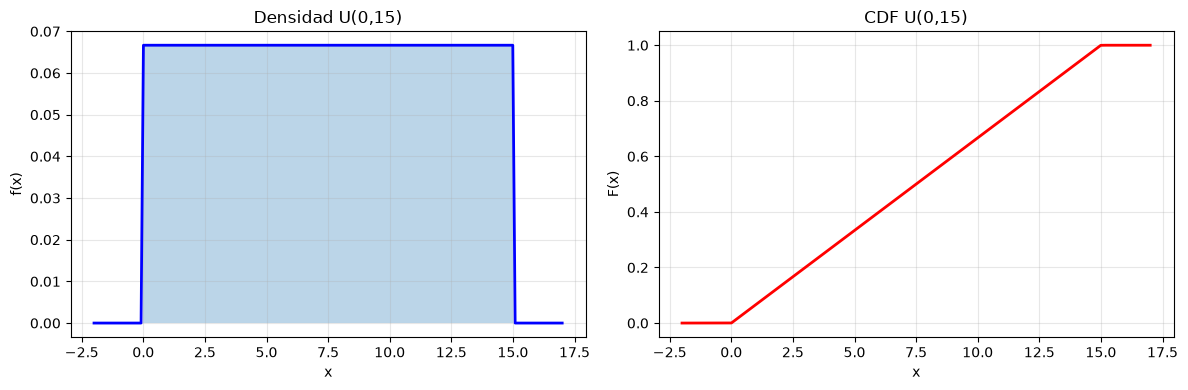
\includegraphics[height=7cm,keepaspectratio=true]{./pe/distUniforme.png}
 % distUniforme.png: 0x0 pixel, 300dpi, 0.00x0.00 cm, bb=
 \caption{Distribuci\'on uniforme continua $U(0,15)$: densidad y CDF.}
 \label{fig:2.8.1}
\end{figure}



\subsection{Distribuci\'on normal}

La distribuci\'on normal es la distribuci\'on continua m\'as importante en estad\'istica
y aparece en el \emph{Teorema del L\'imite Central}.

\begin{definicion}[Distribuci\'on normal]
Una variable aleatoria continua $X$ tiene \emph{distribuci\'on normal} con par\'ametros
$\mu$ (media) y $\sigma > 0$ (desviaci\'on est\'andar) si su funci\'on de densidad es
\begin{align}
 \label{eq:2.8.3}
 f(x) = \frac{1}{\sigma\sqrt{2\pi}}\,\exp\!\left(-\frac{(x-\mu)^2}{2\sigma^2}\right),
 \qquad x \in \mathbb{R}.
\end{align}
Escribimos $X \sim N(\mu, \sigma^2)$.
\end{definicion}

{Propiedades de la distribuci\'on normal} Si $X \sim N(\mu,\sigma^2)$, entonces
\begin{itemize}
 \item La distribuci\'on es \emph{sim\'etrica} respecto a $\mu$.
 \item $\mu$ es la media, mediana y moda.
 \item $\sigma^2$ es la varianza.
 \item Si $Z \sim N(0,1)$ (forma est\'andar), entonces
 $X = \mu + \sigma Z$.
\end{itemize}

{Forma est\'andar} Si $X \sim N(\mu, \sigma^2)$, la variable estandarizada
\begin{align}
 \label{eq:2.8.4}
 Z = \frac{X - \mu}{\sigma}
\end{align}
sigue una distribuci\'on $N(0,1)$ con densidad
\begin{align}
 \label{eq:2.8.5}
 \varphi(z) = \frac{1}{\sqrt{2\pi}}\,e^{-z^2/2}, \qquad z \in \mathbb{R}.
\end{align}

{Regla emp\'irica $68$--$95$--$99.7$} Si $X \sim N(\mu,\sigma^2)$, entonces
\begin{align}
 P(\mu - \sigma \leq X \leq \mu + \sigma) &\approx 0.6827, \\
 P(\mu - 2\sigma \leq X \leq \mu + 2\sigma) &\approx 0.9545, \\
 P(\mu - 3\sigma \leq X \leq \mu + 3\sigma) &\approx 0.9973.
\end{align}

\begin{observacion}
La distribuci\'on normal aparece en muchas situaciones pr\'acticas: errores de medici\'on,
altura de personas, puntajes de ex\'amenes, etc. Adem\'as, por el Teorema del L\'imite
Central, la suma (o promedio) de muchas variables aleatorias independientes (bajo
condiciones suaves) se aproxima a una normal.
\end{observacion}

\begin{ejemplo}
 \label{exmp:2.8.2}
Las calificaciones de un examen siguen una distribuci\'on $N(70, 100)$ (media $70$,
varianza $100$, es decir, $\sigma=10$). ¿Qu\'e porcentaje de estudiantes obtuvo entre
$60$ y $80$ puntos?
\end{ejemplo}

\begin{solucion}
Estandarizamos: si $X \sim N(70, 100)$, entonces
\begin{align}
 P(60 \leq X \leq 80) = P\!\left(\frac{60-70}{10} \leq Z \leq \frac{80-70}{10}\right)
 = P(-1 \leq Z \leq 1).
\end{align}

Por la regla emp\'irica, este valor es aproximadamente $0.6827 = 68.27\%$.
Usando tablas o software, el valor exacto es $\Phi(1) - \Phi(-1) = 0.8413 - 0.1587 = 0.6827$.
\end{solucion}

[fragile, allowframebreaks]{distNormalContinua.py}
 \begin{verbatim}
from scipy import stats
import numpy as np
import matplotlib.pyplot as plt

# Distribuci\'on normal
mu, sigma = 70, 10
normalDist = stats.norm(mu, sigma)

# P(60 <= X <= 80)
p = normalDist.cdf(80) - normalDist.cdf(60)
print(f"P(60 <= X <= 80) = {p:.4f}")
##P(60 <= X <= 80) = 0.6827

# Cuantiles
print(f"Percentil 95: {normalDist.ppf(0.95):.2f}")  # ~86.45
##Percentil 95: 86.45

# Gr\'afica de la densidad con regiones sombreadas
fig, ax = plt.subplots(figsize=(10, 5))
x = np.linspace(mu - 4*sigma, mu + 4*sigma, 500)
ax.plot(x, normalDist.pdf(x), 'b-', lw=2, label=f'N({mu},{sigma**2})')

# Sombrear regi\'on [\mu-\sigma, \mu+\sigma]
x_fill = np.linspace(mu-sigma, mu+sigma, 100)
ax.fill_between(x_fill, normalDist.pdf(x_fill), alpha=0.3, color='blue',
                label='~68.27%')
ax.fill_between(x, normalDist.pdf(x),
                where=((x>=mu-2*sigma)&(x<=mu+2*sigma))&~((x>=mu-sigma)&(x<=mu+sigma)),
                alpha=0.2, color='green', label='~95.45% total')

ax.set_xlabel('x')
ax.set_ylabel('f(x)')
ax.set_title('Distribuci\'on N(70, 100) con regla 68-95-99.7')
ax.legend(loc='upper right')
ax.grid(True, alpha=0.3)
plt.tight_layout()
plt.savefig('pe/distNormalContinua.png', dpi=100, bbox_inches='tight')
plt.show()
 \end{verbatim}

\begin{figure}
 \centering
 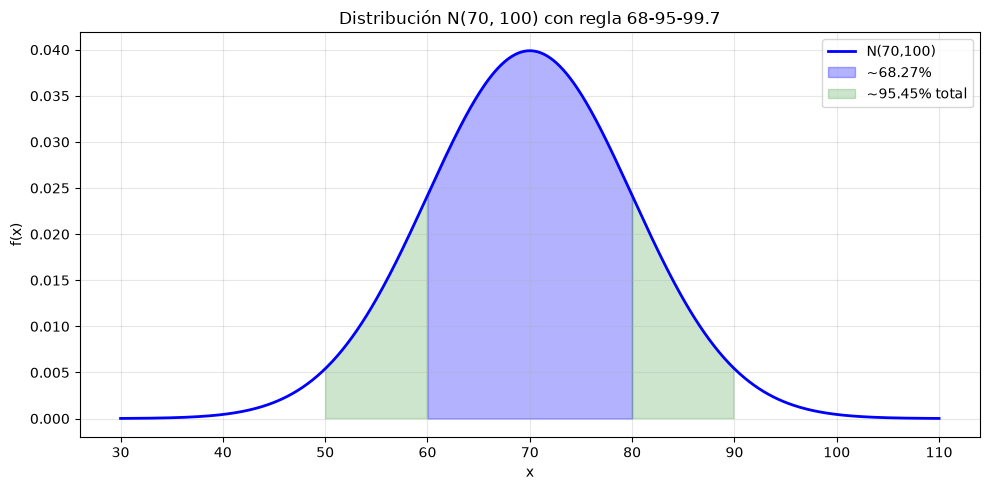
\includegraphics[height=7cm,keepaspectratio=true]{./pe/distNormalContinua.png}
 % distNormalContinua.png: 0x0 pixel, 300dpi, 0.00x0.00 cm, bb=
 \caption{Distribuci\'on $N(70,100)$ mostrando la regla emp\'irica 68--95--99.7.}
 \label{fig:2.8.2}
\end{figure}



\subsection{Distribuciones de tipo gamma}

La familia gamma es una generalizaci\'on de varias distribuciones importantes
(exponencial, chi-cuadrada, Erlang) y aparece frecuentemente al modelar
\emph{tiempos de espera}.

\subsubsection{Funci\'on gamma}

\begin{definicion}[Funci\'on gamma]
La \emph{funci\'on gamma} $\Gamma: (0,\infty) \to \mathbb{R}$ se define como
\begin{align}
 \label{eq:2.8.6}
 \Gamma(\alpha) = \int_0^\infty t^{\alpha-1} e^{-t}\,dt.
\end{align}
\end{definicion}

{Propiedades de la funci\'on gamma}
\begin{itemize}
 \item $\Gamma(1) = 1$.
 \item $\Gamma(\alpha + 1) = \alpha\,\Gamma(\alpha)$ para todo $\alpha > 0$.
 \item En particular, para $\alpha \in \mathbb{N}$ se cumple
 $\Gamma(n) = (n-1)!$.
 \item $\Gamma(1/2) = \sqrt{\pi}$.
\end{itemize}

\subsubsection{Distribuci\'on gamma}

\begin{definicion}[Distribuci\'on gamma]
Una variable aleatoria continua $X$ tiene \emph{distribuci\'on gamma} con par\'ametros
de forma $\alpha > 0$ y escala $\beta > 0$ si su funci\'on de densidad es
\begin{align}
 \label{eq:2.8.7}
 f(x) =
 \begin{cases}
  \dfrac{1}{\Gamma(\alpha)\,\beta^\alpha}\,x^{\alpha-1}\,e^{-x/\beta},
  & x > 0, \\
  0, & \text{en otro caso.}
 \end{cases}
\end{align}
Escribimos $X \sim \text{Gamma}(\alpha, \beta)$.
\end{definicion}

{Propiedades de la distribuci\'on gamma} Si $X \sim \text{Gamma}(\alpha, \beta)$, entonces
\begin{align}
 \mu_X &= \alpha\beta, \\
 \s_X^2 &= \alpha\beta^2.
\end{align}

\subsubsection{Caso particular: distribuci\'on exponencial ($\alpha = 1$)}

\begin{definicion}[Distribuci\'on exponencial]
Una variable aleatoria $X$ con distribuci\'on $\text{Gamma}(1, \beta)$ se dice que
tiene \emph{distribuci\'on exponencial} con par\'ametro $\lambda = 1/\beta$. Su
funci\'on de densidad es
\begin{align}
 \label{eq:2.8.8}
 f(x) =
 \begin{cases}
  \lambda\,e^{-\lambda x}, & x \geq 0, \\
  0, & \text{en otro caso.}
 \end{cases}
\end{align}
Su media y varianza son $\mu = 1/\lambda$ y $\sigma^2 = 1/\lambda^2$.
\end{definicion}

\begin{observacion}[Propiedad de p\'erdida de memoria]
La distribuci\'on exponencial satisface la \emph{propiedad de p\'erdida de memoria}:
para $s, t \geq 0$,
\begin{align}
 P(X > s + t \mid X > s) = P(X > t).
\end{align}
Es la \'unica distribuci\'on continua (adem\'as de la geom\'etrica en el caso discreto)
con esta propiedad.
\end{observacion}

\subsubsection{Caso particular: distribuci\'on chi-cuadrada}

La distribuci\'on chi-cuadrada con $\nu$ grados de libertad, denotada $\chi^2_\nu$, es
un caso particular de la distribuci\'on gamma con par\'ametros
$\alpha = \nu/2$ y $\beta = 2$:
\begin{align}
 \label{eq:2.8.9}
 X \sim \chi^2_\nu \iff X \sim \text{Gamma}\!\left(\frac{\nu}{2}, 2\right).
\end{align}
Su funci\'on de densidad es
\begin{align}
 f(x) = \frac{1}{2^{\nu/2}\,\Gamma(\nu/2)}\,x^{\nu/2-1}\,e^{-x/2}, \qquad x > 0.
\end{align}

Esta distribuci\'on ya se estudia en detalle en la secci\'on \ref{sec:3.8} del cap\'itulo
de inferencia; la conexi\'on con la familia gamma permite generalizar varios de sus
resultados.

\subsubsection{Suma de variables gamma independientes}

\begin{teorema}[Propiedad de suma de gamma]
Si $X_1, X_2, \dots, X_n$ son variables aleatorias independientes con
$X_i \sim \text{Gamma}(\alpha_i, \beta)$ (con la misma escala $\beta$), entonces
\begin{align}
 \label{eq:2.8.10}
 Y = X_1 + X_2 + \cdots + X_n \sim \text{Gamma}\!\left(\sum_{i=1}^n \alpha_i,\, \beta\right).
\end{align}
\end{teorema}

\begin{ejemplo}
 \label{exmp:2.8.3}
Las llamadas a un \emph{call center} llegan siguiendo un proceso de Poisson con tasa
$\lambda = 3$ llamadas por minuto. ¿Cu\'al es la distribuci\'on del tiempo hasta la
tercera llamada? ¿Cu\'al es la probabilidad de que este tiempo sea mayor a $1.5$ minutos?
\end{ejemplo}

\begin{solucion}
El tiempo entre llamadas consecutivas es exponencial con par\'ametro $\lambda = 3$, es
decir, $T_i \sim \text{Exp}(3)$ con media $1/3$ minutos.

Por la propiedad aditiva de la distribuci\'on gamma, el tiempo hasta la tercera llamada
es
\begin{align}
 T = T_1 + T_2 + T_3 \sim \text{Gamma}(3, 1/3).
\end{align}
Equivalentemente, $T \sim \text{Erlang}(3, 3)$ con par\'ametro de tasa $3$.

La probabilidad de que $T > 1.5$ es
\begin{align}
 P(T > 1.5) = 1 - F_{\text{Gamma}}(1.5; 3, 1/3) = e^{-3 \cdot 1.5}\left(1 + 3\cdot 1.5 + \frac{(3\cdot 1.5)^2}{2}\right).
\end{align}

Num\'ericamente: $3 \cdot 1.5 = 4.5$, por lo que
\begin{align}
 P(T > 1.5) = e^{-4.5}\left(1 + 4.5 + \frac{20.25}{2}\right) = e^{-4.5}(15.625) \approx 0.174.
\end{align}
\end{solucion}

[fragile, allowframebreaks]{distGamma.py}
 \begin{verbatim}
from scipy import stats
import numpy as np
import matplotlib.pyplot as plt

# Distribuci\'on gamma con varios par\'ametros
fig, axes = plt.subplots(1, 2, figsize=(14, 5))

# Panel izquierdo: variando alpha (beta=1 fijo)
x = np.linspace(0, 15, 500)
alphas = [1, 2, 3, 5]
for a in alphas:
    g = stats.gamma(a=a, scale=1.0)
    axes[0].plot(x, g.pdf(x), lw=2, label=f'alpha={a}, beta=1')

axes[0].set_xlabel('x')
axes[0].set_ylabel('f(x)')
axes[0].set_title('Familia gamma (variando alpha)')
axes[0].legend()
axes[0].grid(True, alpha=0.3)

# Panel derecho: distribuciones exponencial y chi-cuadrada como casos particulares
x2 = np.linspace(0, 10, 500)
exp_dist = stats.expon(scale=1.0)              # Gamma(alpha=1, beta=1)
chi2_3 = stats.chi2(df=3)                      # Gamma(alpha=1.5, beta=2)
chi2_5 = stats.chi2(df=5)                      # Gamma(alpha=2.5, beta=2)

axes[1].plot(x2, exp_dist.pdf(x2), 'b-', lw=2, label='Exp(1) = Gamma(1,1)')
axes[1].plot(x2, chi2_3.pdf(x2), 'r-', lw=2, label='chi^2_3 = Gamma(1.5,2)')
axes[1].plot(x2, chi2_5.pdf(x2), 'g-', lw=2, label='chi^2_5 = Gamma(2.5,2)')
axes[1].set_xlabel('x')
axes[1].set_ylabel('f(x)')
axes[1].set_title('Exponencial y chi-cuadrada como casos de gamma')
axes[1].legend()
axes[1].grid(True, alpha=0.3)

plt.tight_layout()
plt.savefig('pe/distGamma.png', dpi=100, bbox_inches='tight')
plt.show()

# Ejemplo: tiempo hasta la tercera llamada
# Erlang(k, lambda) = Gamma(k, 1/lambda)
lam = 3
k = 3
T = stats.gamma(a=k, scale=1/lam)
print(f"P(T > 1.5) = {1 - T.cdf(1.5):.4f}")
##P(T > 1.5) = 0.1739

# Simulaci\'on
np.random.seed(0)
muestras = np.random.gamma(shape=k, scale=1/lam, size=10000)
print(f"Media muestral: {np.mean(muestras):.4f}")  # Esperado: 1
##Media muestral: 1.0036
 \end{verbatim}

\begin{figure}
 \centering
 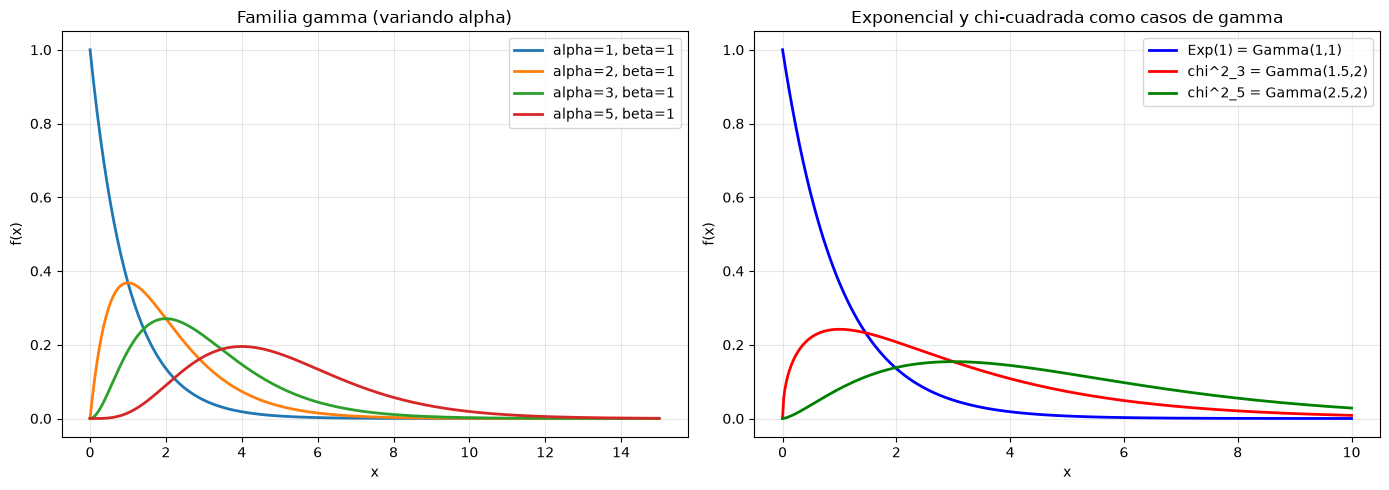
\includegraphics[height=7cm,keepaspectratio=true]{./pe/distGamma.png}
 % distGamma.png: 0x0 pixel, 300dpi, 0.00x0.00 cm, bb=
 \caption{Familia gamma y sus casos particulares (exponencial y chi-cuadrada).}
 \label{fig:2.8.3}
\end{figure}



\subsection{Funci\'on generadora de momentos}

La funci\'on generadora de momentos (FGM) es una herramienta que codifica toda la
informaci\'on de una distribuci\'on de probabilidad en una \'unica funci\'on.

\begin{definicion}[Funci\'on generadora de momentos]
Sea $X$ una variable aleatoria. Su \emph{funci\'on generadora de momentos} (FGM) es
\begin{align}
 \label{eq:2.8.11}
 M_X(t) = E\!\left[e^{tX}\right].
\end{align}
Si $X$ es discreta con funci\'on de probabilidad $f$,
\begin{align}
 M_X(t) = \sum_x e^{tx} f(x).
\end{align}
Si $X$ es continua con funci\'on de densidad $f$,
\begin{align}
 M_X(t) = \int_{-\infty}^{\infty} e^{tx} f(x)\,dx.
\end{align}
\end{definicion}

La FGM existe si la integral o suma converge en un entorno abierto de $t=0$.

\subsubsection{Momentos a partir de la FGM}

\begin{teorema}[Derivadas y momentos]
Si $M_X(t)$ es la FGM de $X$, entonces para todo $n \in \mathbb{N}$,
\begin{align}
 \label{eq:2.8.12}
 E\!\left[X^n\right] = M_X^{(n)}(0) = \left.\frac{d^n M_X(t)}{dt^n}\right|_{t=0}.
\end{align}
\end{teorema}

\begin{proof}
Intercambiando derivada y esperanza (bajo condiciones de regularidad):
\begin{align}
 M_X^{(n)}(t) = \frac{d^n}{dt^n}E[e^{tX}] = E\!\left[\frac{d^n}{dt^n}e^{tX}\right]
 = E\!\left[X^n e^{tX}\right].
\end{align}
Evaluando en $t=0$ obtenemos $M_X^{(n)}(0) = E[X^n]$.
\end{proof}

\subsubsection{Unicidad y propiedad de suma}

\begin{teorema}[Unicidad]
Si dos variables aleatorias tienen la misma FGM en un entorno de $t=0$, entonces tienen
la misma distribuci\'on de probabilidad.
\end{teorema}

\begin{teorema}[Propiedad de suma]
Si $X$ e $Y$ son variables aleatorias independientes, entonces
\begin{align}
 \label{eq:2.8.13}
 M_{X+Y}(t) = M_X(t)\,M_Y(t).
\end{align}
\end{teorema}

\begin{proof}
Por independencia,
\begin{align}
 M_{X+Y}(t) = E[e^{t(X+Y)}] = E[e^{tX}e^{tY}] = E[e^{tX}]\,E[e^{tY}] = M_X(t)\,M_Y(t).
\end{align}
\end{proof}

\subsubsection{Ejemplos de FGM}

\begin{ejemplo}
 \label{exmp:2.8.4}
Encuentre la FGM de la distribuci\'on Bernoulli con par\'ametro $p$.
\end{ejemplo}

\begin{solucion}
Si $X \sim \text{Bernoulli}(p)$, entonces $P(X=1) = p$ y $P(X=0) = 1-p$.
\begin{align}
 M_X(t) = E[e^{tX}] = e^{0 \cdot t}(1-p) + e^{1 \cdot t}p
 = (1-p) + p\,e^t.
\end{align}

Verificamos los momentos:
\begin{align}
 M_X'(t) = p\,e^t &\implies E[X] = M_X'(0) = p. \\
 M_X''(t) = p\,e^t &\implies E[X^2] = M_X''(0) = p. \\
 \text{Var}(X) = E[X^2] - (E[X])^2 &= p - p^2 = p(1-p).
\end{align}
\end{solucion}

\begin{ejemplo}
 \label{exmp:2.8.5}
Encuentre la FGM de la distribuci\'on normal $N(\mu, \sigma^2)$.
\end{ejemplo}

\begin{solucion}
Sin p\'erdida de generalidad, considere $Z \sim N(0,1)$. Entonces
\begin{align}
 M_Z(t) &= \int_{-\infty}^{\infty} e^{tz}\,\frac{1}{\sqrt{2\pi}}e^{-z^2/2}\,dz \\
 &= \int_{-\infty}^{\infty} \frac{1}{\sqrt{2\pi}}\,\exp\!\left(tz - \frac{z^2}{2}\right)dz.
\end{align}

Completamos el cuadrado: $tz - z^2/2 = -\frac{1}{2}(z - t)^2 + \frac{t^2}{2}$. Por lo tanto,
\begin{align}
 M_Z(t) = e^{t^2/2}\int_{-\infty}^{\infty} \frac{1}{\sqrt{2\pi}}e^{-(z-t)^2/2}\,dz = e^{t^2/2}.
\end{align}
(la integral vale $1$ porque es la integral de la densidad de $N(t, 1)$).

Para $X \sim N(\mu,\sigma^2)$ escribimos $X = \mu + \sigma Z$, as\'i
\begin{align}
 \label{eq:2.8.14}
 M_X(t) = E[e^{tX}] = e^{t\mu}E[e^{t\sigma Z}] = e^{t\mu}\,e^{(\sigma t)^2/2}
 = \exp\!\left(\mu t + \frac{\sigma^2 t^2}{2}\right).
\end{align}
\end{solucion}

\begin{ejemplo}
 \label{exmp:2.8.6}
Encuentre la FGM de la distribuci\'on exponencial con par\'ametro $\lambda$.
\end{ejemplo}

\begin{solucion}
Si $X \sim \text{Exp}(\lambda)$, entonces
\begin{align}
 M_X(t) = \int_0^\infty e^{tx}\,\lambda e^{-\lambda x}\,dx
 = \lambda\int_0^\infty e^{-(\lambda - t)x}\,dx = \frac{\lambda}{\lambda - t},
\end{align}
para $t < \lambda$. Por lo tanto,
\begin{align}
 \label{eq:2.8.15}
 M_X(t) = \frac{\lambda}{\lambda - t} = \left(1 - \frac{t}{\lambda}\right)^{-1},
 \qquad t < \lambda.
\end{align}

Los momentos se obtienen por derivaci\'on:
\begin{align}
 E[X^n] = \frac{n!}{\lambda^n}.
\end{align}
En particular, $E[X] = 1/\lambda$ y $\text{Var}(X) = 1/\lambda^2$.
\end{solucion}

[fragile, allowframebreaks]{fgmDistribuciones.py}
 \begin{verbatim}
import numpy as np
import matplotlib.pyplot as plt
from scipy import stats

fig, axes = plt.subplots(1, 2, figsize=(14, 5))

# Panel izquierdo: FGM de varias distribuciones
t = np.linspace(-1.5, 1.5, 200)

# Bernoulli(0.5)
M_bernoulli = lambda t: 0.5 + 0.5*np.exp(t)
axes[0].plot(t, M_bernoulli(t), label='Bernoulli(0.5)', lw=2)

# Normal(0,1)
M_normal = lambda t: np.exp(t**2 / 2)
axes[0].plot(t, M_normal(t), label='N(0,1)', lw=2)

# Exponencial(lambda=1)
lam = 1
M_exp = lambda t: lam / (lam - t)
mask = t < lam - 0.01
axes[0].plot(t[mask], M_exp(t[mask]), label='Exp(1)', lw=2)

# Gamma(2, 1) = Erlang(2, 1)
# M(t) = (1 - t)^(-alpha) para beta=1
M_gamma = lambda t: (1 - t)**(-2)
mask_g = t < 0.99
axes[0].plot(t[mask_g], M_gamma(t[mask_g]), label='Gamma(2,1)', lw=2)

axes[0].set_xlabel('t')
axes[0].set_ylabel('M_X(t)')
axes[0].set_title('Funciones generadoras de momentos')
axes[0].set_ylim(-1, 8)
axes[0].legend()
axes[0].grid(True, alpha=0.3)
axes[0].axhline(y=0, color='k', lw=0.5)
axes[0].axvline(x=0, color='k', lw=0.5)

# Panel derecho: verificaci\'on de momentos de N(0,1)
X = np.random.normal(0, 1, 100000)
momentos_empiricos = [np.mean(X**k) for k in range(1, 6)]
print("Momentos emp\'iricos de N(0,1):", momentos_empiricos)
# Esperado: 0, 1, 0, 3, 0  (solo momentos pares son no cero)
##Momentos emp\'iricos de N(0,1): [0.001, 0.998, -0.001, 2.978, -0.011]

# FGM: suma de gamma independientes
# Si X_i ~ Gamma(1, 1) iid, entonces sum = Gamma(n, 1)
n_sumas = [1, 2, 5, 10]
x = np.linspace(0, 20, 200)
for n in n_sumas:
    g = stats.gamma(a=n, scale=1.0)
    axes[1].plot(x, g.pdf(x), lw=2, label=f'suma de {n} Exp(1)')
axes[1].set_xlabel('x')
axes[1].set_ylabel('f(x)')
axes[1].set_title('Suma de exponenciales = Erlang(Gamma)')
axes[1].legend()
axes[1].grid(True, alpha=0.3)

plt.tight_layout()
plt.savefig('pe/fgmDistribuciones.png', dpi=100, bbox_inches='tight')
plt.show()
 \end{verbatim}

\begin{figure}
 \centering
 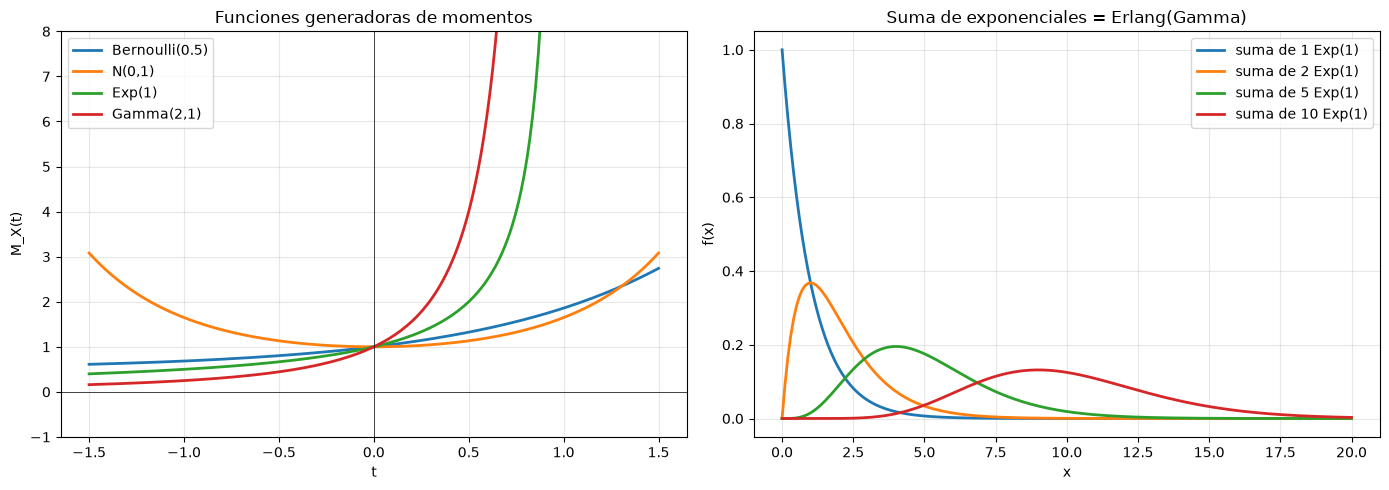
\includegraphics[height=7cm,keepaspectratio=true]{./pe/fgmDistribuciones.png}
 % fgmDistribuciones.png: 0x0 pixel, 300dpi, 0.00x0.00 cm, bb=
 \caption{Funciones generadoras de momentos y suma de variables gamma independientes.}
 \label{fig:2.8.4}
\end{figure}

{Tabla resumen de FGMs}
\begin{center}
\begin{tabular}{|l|l|}
\hline
\textbf{Distribuci\'on} & \textbf{FGM $M_X(t)$} \\
\hline
Bernoulli$(p)$ & $(1-p) + p\,e^t$ \\
Binomial$(n,p)$ & $(1 - p + p\,e^t)^n$ \\
Poisson$(\lambda)$ & $\exp(\lambda(e^t - 1))$ \\
Geom\'etrica$(p)$ & $\dfrac{p\,e^t}{1 - (1-p)e^t}$ \\
Exponencial$(\lambda)$ & $\dfrac{\lambda}{\lambda - t}$ \\
Normal$(\mu, \sigma^2)$ & $\exp\!\left(\mu t + \dfrac{\sigma^2 t^2}{2}\right)$ \\
Gamma$(\alpha, \beta)$ & $(1 - \beta t)^{-\alpha}$ \\
Chi-cuadrada$_\nu$ & $(1 - 2t)^{-\nu/2}$ \\
\hline
\end{tabular}
\end{center}

\begin{observacion}
La propiedad de suma para v.a. independientes se aplica f\'acilmente: si
$X_1, \dots, X_n$ son Bernoulli$(p)$ iid, entonces
$\sum X_i \sim \text{Binomial}(n,p)$ y
\begin{align}
 M_{\sum X_i}(t) = \prod_{i=1}^n M_{X_i}(t) = (1 - p + p\,e^t)^n,
\end{align}
que coincide con la FGM de la distribuci\'on binomial.
\end{observacion}



